
\begin{frame}{Entropy}
	\begin{block}{Measure of Disorder... Or Energy... Or Information}
		\begin{itemize}
		 	\item Boltzmann Entropy: $S_B = k\ln(w)$
		 	\item Gibbs Entropy: $S_G = -k\sum_i P_i \ln(P_i)$
		 	\item Shannon Entropy: $\shannon = -\sum_i P_i \ln(P_i)$
		\end{itemize}
	\end{block}
\end{frame}

\begin{frame}{Entropy}
\begin{figure}
	\centering
	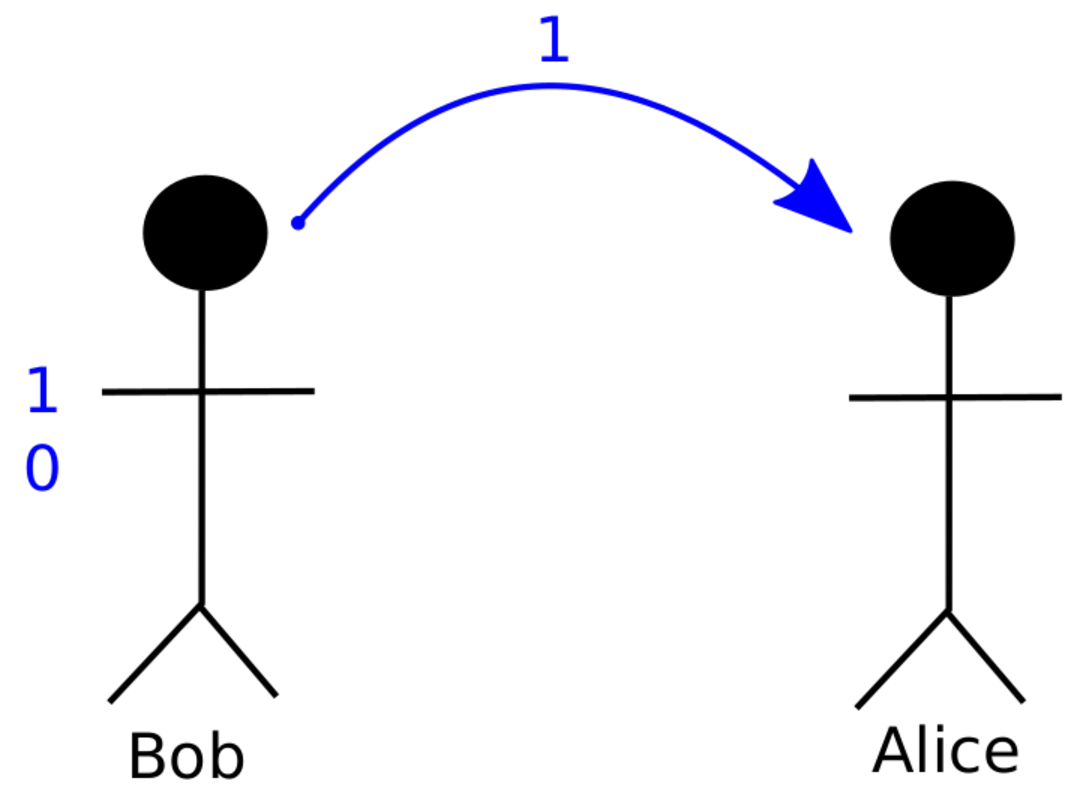
\includegraphics[height=2.5cm]{alice_and_bob.pdf}
	\caption{A tale as old as time.}
	\label{fig:alice_and_bob}
\end{figure}
\begin{block}{Information Content}
\begin{itemize}
	\item How much information does Bob's message give Alice?
	\item More quantitatively, given $\Gamma := \{0,1\}$
	\begin{equation*}
		I: \Gamma \to \R
	\end{equation*}
\end{itemize}
\end{block}
\end{frame}

\begin{frame}{Entropy}
\begin{block}{Case 1}
\begin{figure}
	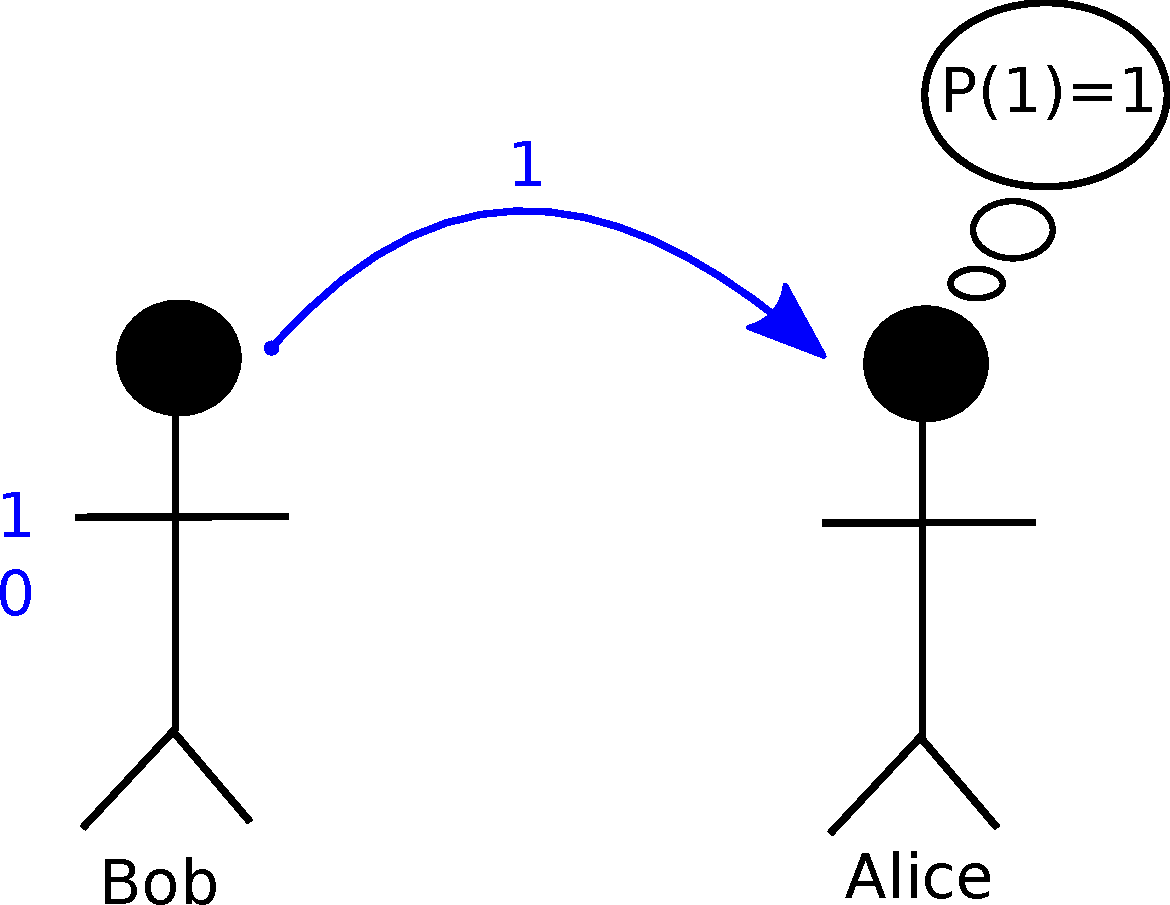
\includegraphics[height=3cm] {alice_and_bob_s1.pdf}
	\label{fig:alice_and_bob_s1}
\end{figure}
\end{block}
\end{frame}

\begin{frame}{Entropy}
\begin{block}{Case 1 cont.}
\begin{figure}
	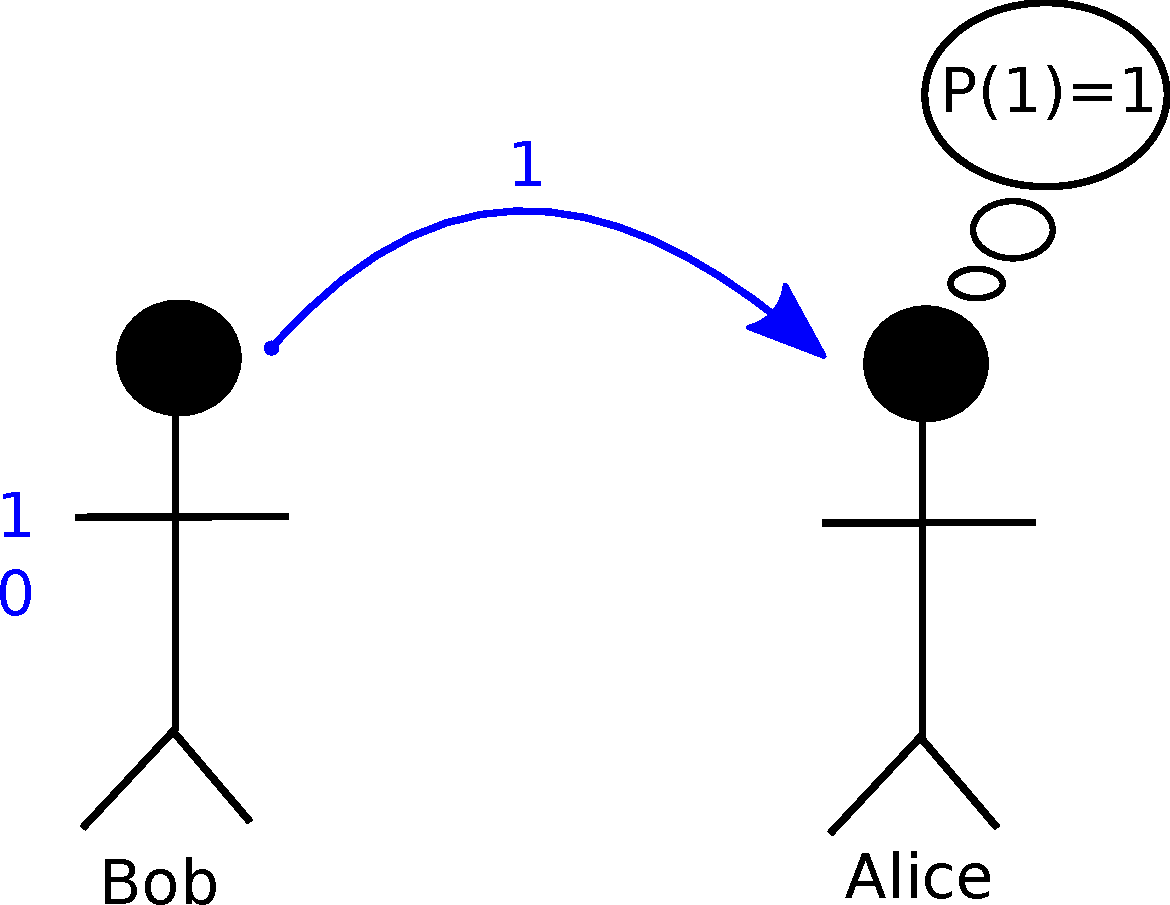
\includegraphics[height=3cm] {alice_and_bob_s1.pdf}
	\label{fig:alice_and_bob_s1_1}
\end{figure}
\begin{itemize}
	\item Bob's message provides no information.
	\item $I(1) = 0$
\end{itemize}
\end{block}
\end{frame}

\begin{frame}{Entropy}
\begin{block}{Case 2}
\begin{figure}
	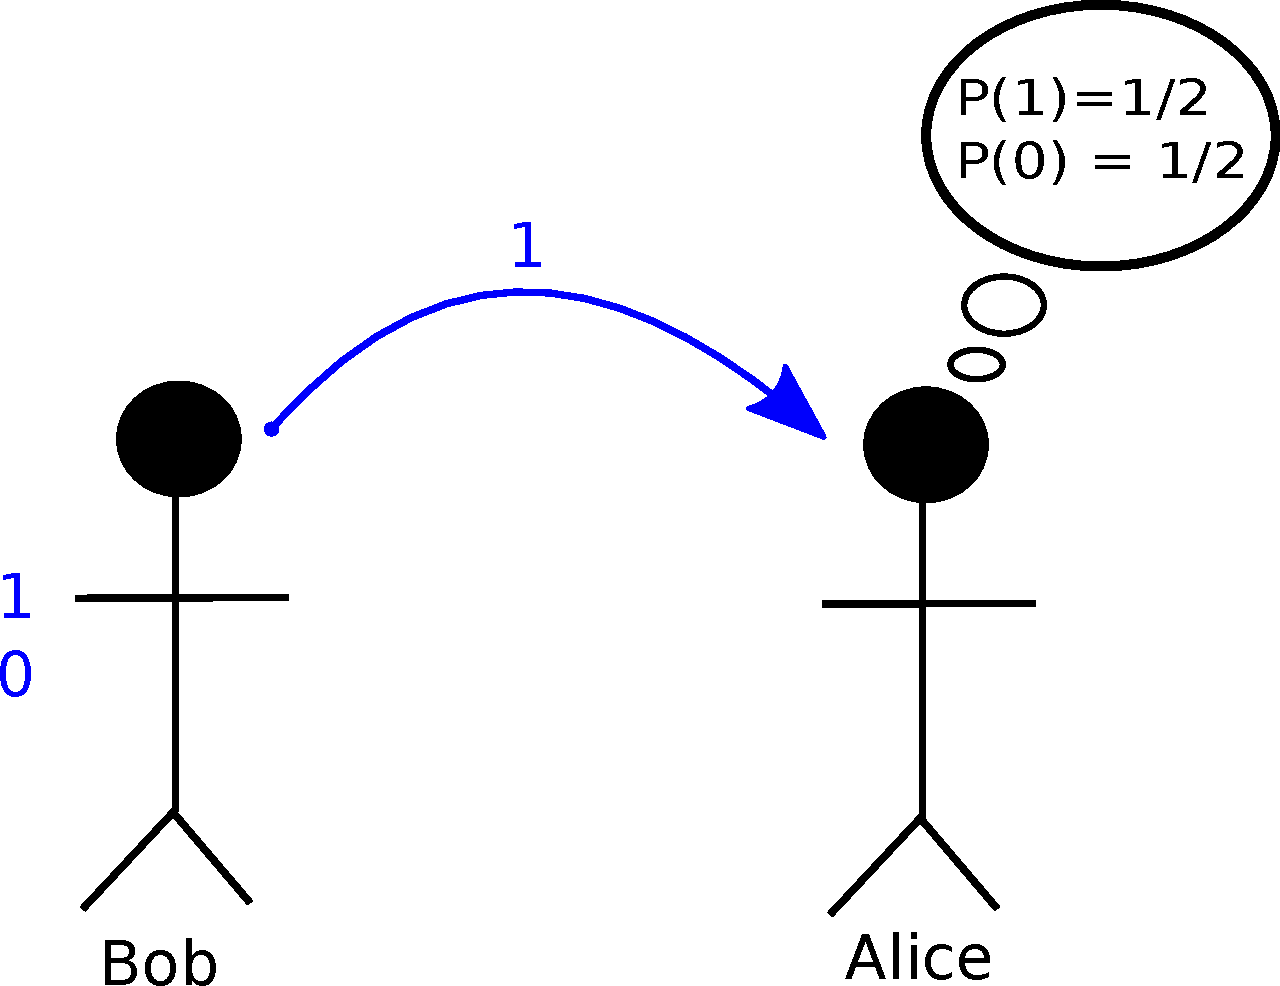
\includegraphics[height=3cm] {alice_and_bob_s2.pdf}
	\label{fig:alice_and_bob_s2}
\end{figure}
\end{block}
\end{frame}


\begin{frame}{Entropy}
\begin{block}{Case 2 cont.}
\begin{figure}
	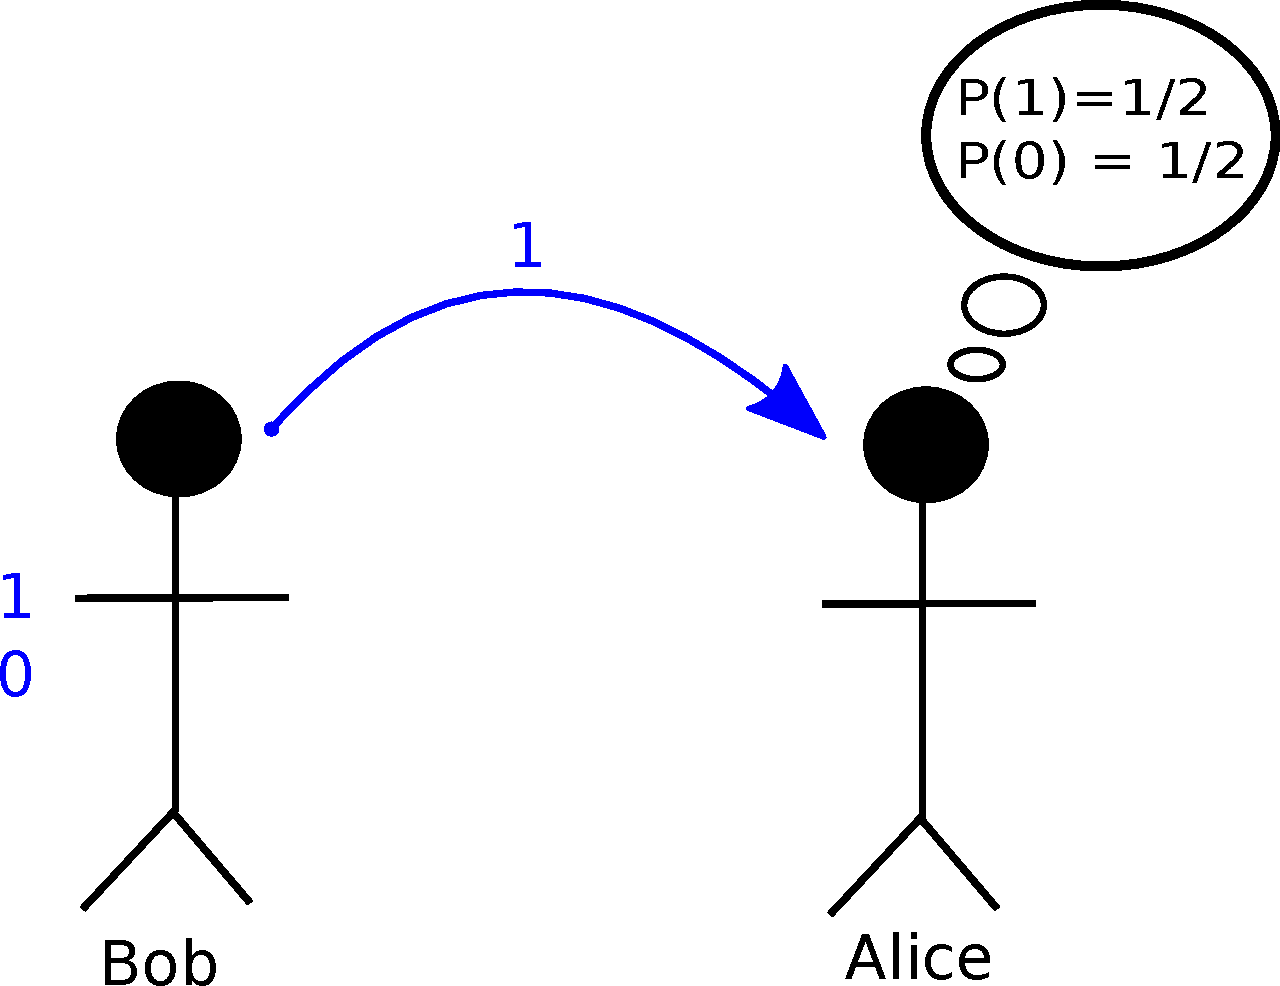
\includegraphics[height=3cm] {alice_and_bob_s2.pdf}
	\label{fig:alice_and_bob_s2_1}
\end{figure}
\begin{itemize}
	\item Bob's message provides one bit of information
	\item $0<I(1)= 1$bit
\end{itemize}
\end{block}
\end{frame}

\begin{frame}{Entropy}
\begin{block}{Case3}
\begin{figure}
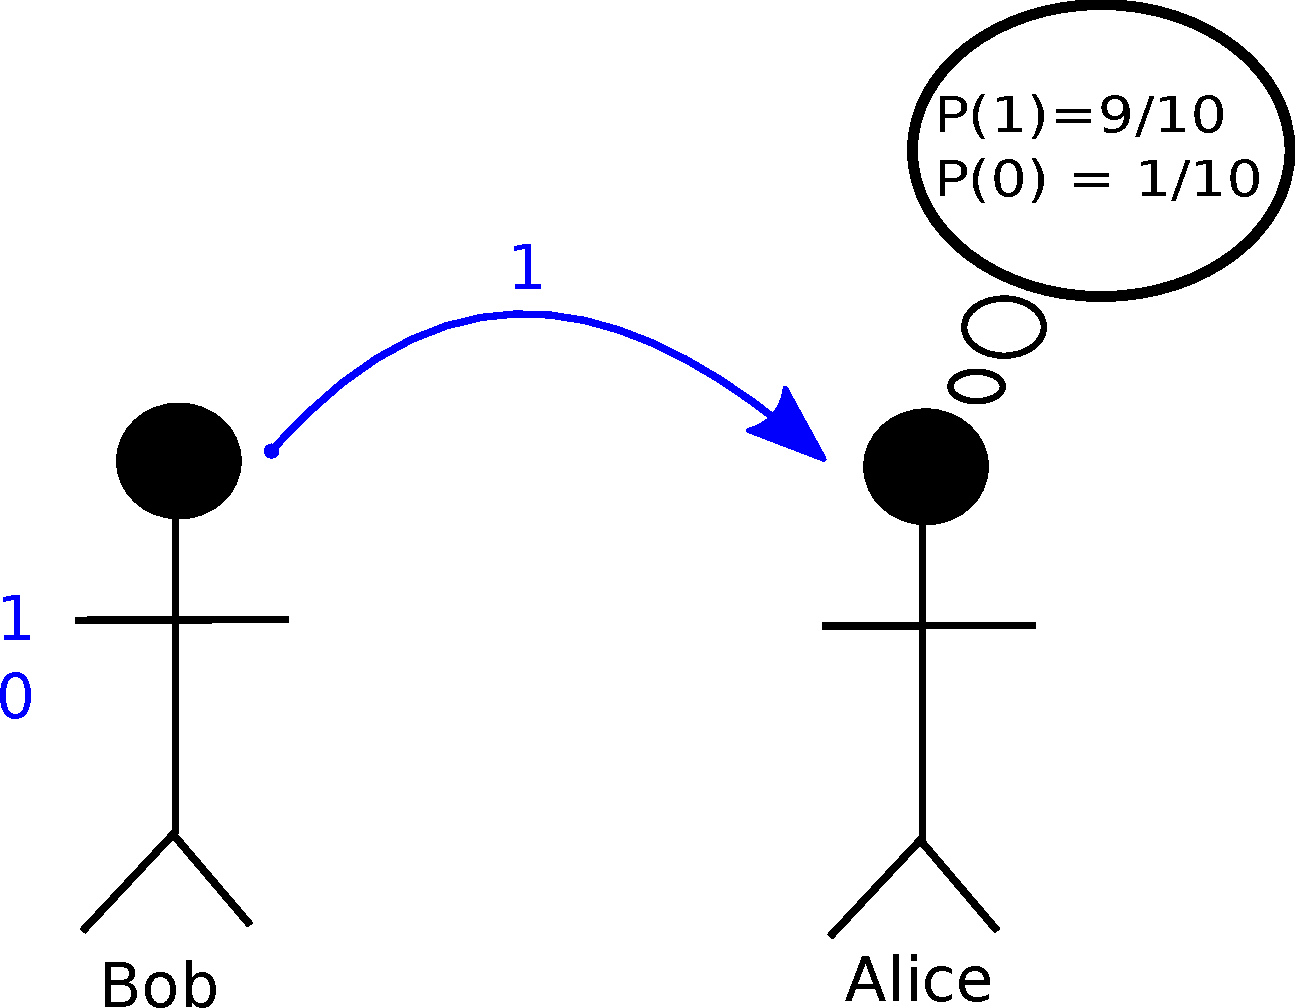
\includegraphics[height=3cm]{alice_and_bob_s3.pdf}
\label{fig:alice_and_bob_s3}
\end{figure}
\end{block}
\end{frame}

\begin{frame}{Entropy}
\begin{block}{Case 3}
\begin{figure}
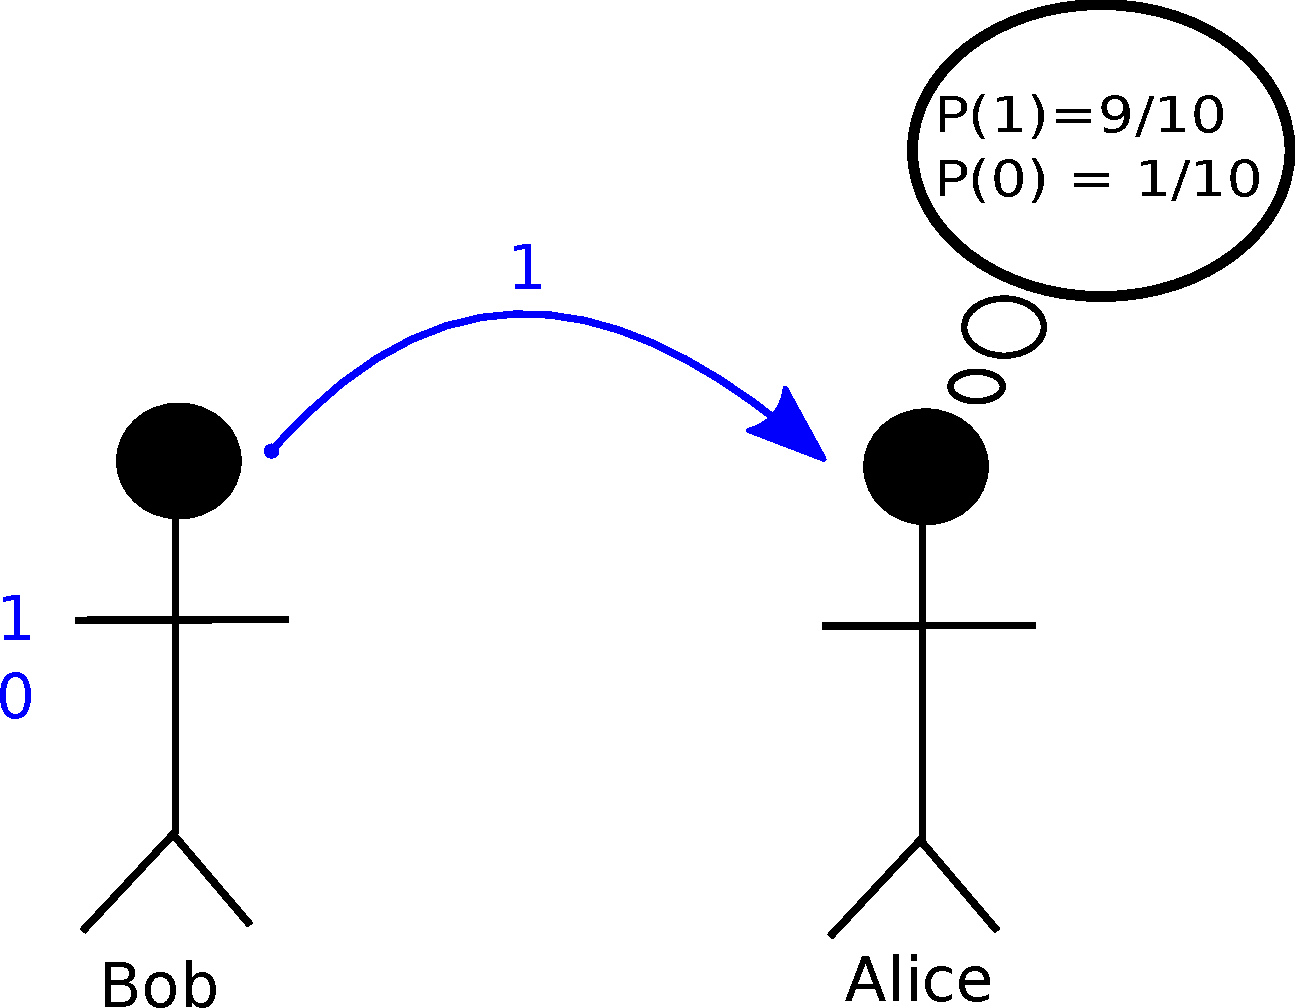
\includegraphics[height=3cm]{alice_and_bob_s3.pdf}
\label{fig:alice_and_bob_s3_1}
\end{figure}
\begin{itemize}
	\item Bob's message removes some uncertainty
	\item Not as informative as in case 2
	\item $0=I^{(1)}(1) < I^{(3)}(1) < I^{(2)}(1)= 1$bit
\end{itemize}
\end{block}
\end{frame}

\begin{frame}{Entropy}
\begin{block}{Case 4}
\begin{figure}
\centering
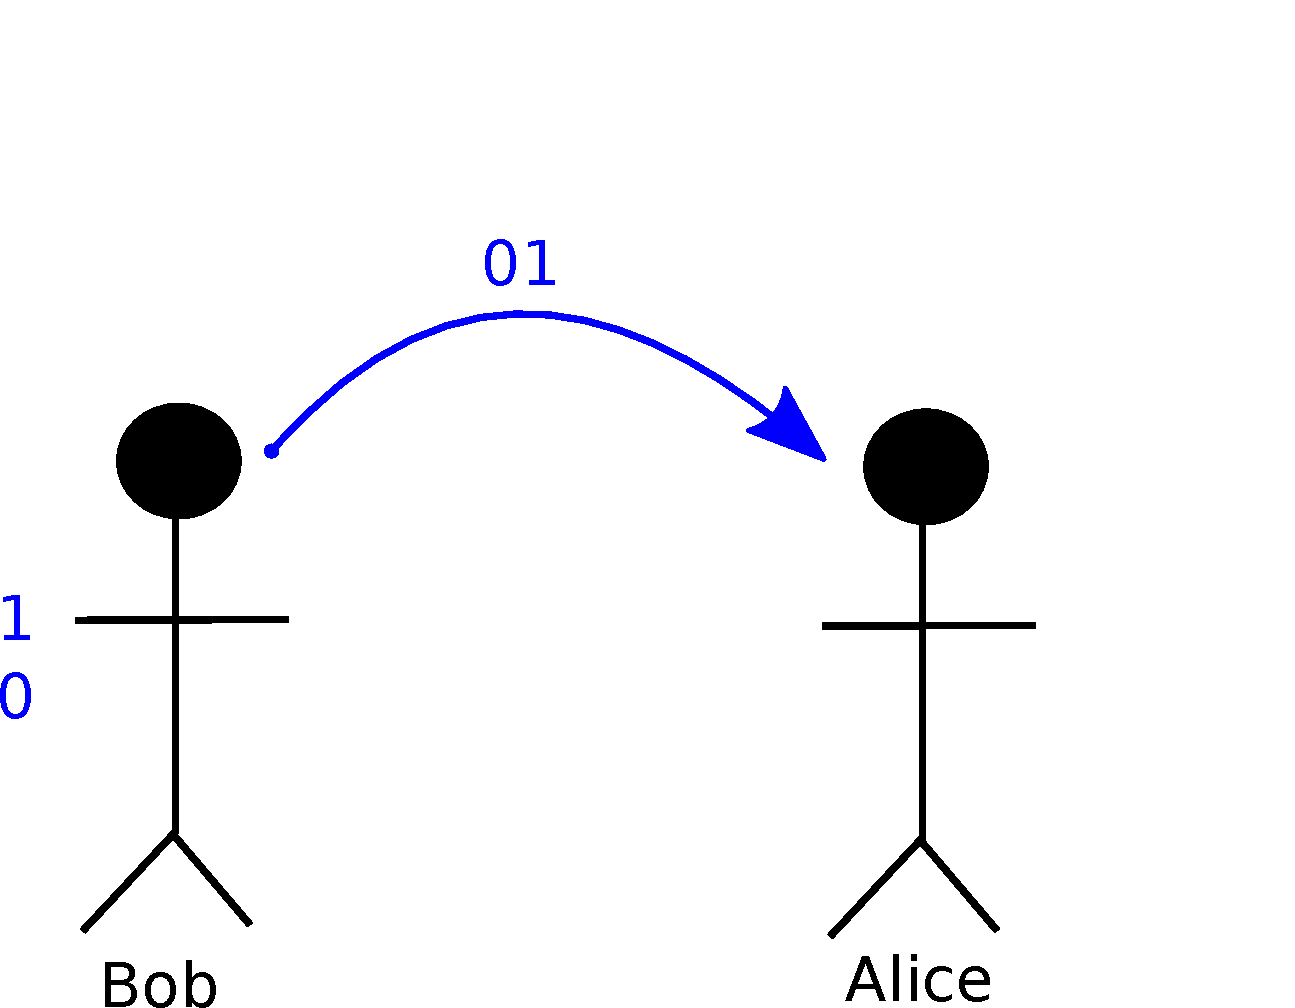
\includegraphics[height=4cm]{alice_and_bob_s4.pdf}
\label{fig:alice_and_bob_s4}
\end{figure}
\begin{itemize}
	\item Decision to send 0 independent from decision to send 1
	\item $I(0,1) = I(0) + I(1)$
\end{itemize}
\end{block}
\end{frame}

\begin{frame}{Entropy}

\begin{block}{ Three Conditions}
For any $x,y \in \Gamma$, the following three axioms must hold:
\begin{enumerate}
	\item $P(x) = 1 \; \implies \; I(x)=0$
	\item $P(x) < P(y) \; \implies \; I(y) < I(x)$
	\item $I(xy) = I(x) + I(y)$
\end{enumerate}
\end{block}
\end{frame}

\begin{frame}{Entropy}
\begin{block}{Information Content, or Surprisal}
Single function which can satisfy these three axioms \parencite{shannon_mathematical_nodate}
\begin{equation*}
I(x) = -\log_b(P_x)
\end{equation*}
Where we write $P_x=P(x)$ for notational simplicity.
\begin{itemize}
	\item This value is called the \textbf{Surprisal}, or \textbf{Information Content}
	\item $b$ sets our units of information
\end{itemize}
\end{block}
\end{frame}

\begin{frame}{Entropy}
\begin{block}{The Bit: $b=2$}
\begin{itemize}
\item If $P(1)=P(2) = 1/2$, then $I(1)=1$ bit.
\begin{align*}
	I_2(1) &= -\log_2(P_1)\\
	&= - \log_2\left(\frac{1}{2}\right)\\
	&= 1
\end{align*}
\end{itemize}
\end{block}
\end{frame}

\begin{frame}{Entropy}
\begin{block}{The nat: $b=e$}
\begin{itemize}
	\item Recall the Boltzmann Entropy $S_B$:
	\begin{equation*}
		S_B = k\ln (w)
	\end{equation*}
	\item $P(w_0) = 1/w$. Thus
	\begin{align*}
		S_B &= -k\ln(P_{w_0})\\
		&= kI_e(w_0)
	\end{align*}
\end{itemize}
\end{block}
\end{frame}

\begin{frame}{Entropy}
\begin{block}{Unit Conversions}
	All $I_b$ are related by the logarithm change-of-base formula:
	\begin{equation*}
	I_c = \frac{1}{\log_b c} I_b
	\end{equation*}
	the factor $\frac{1}{\log_b c}$ can be thought of as a conversion factor.
\end{block}
\end{frame}




\begin{frame}{Entropy}
\begin{figure}
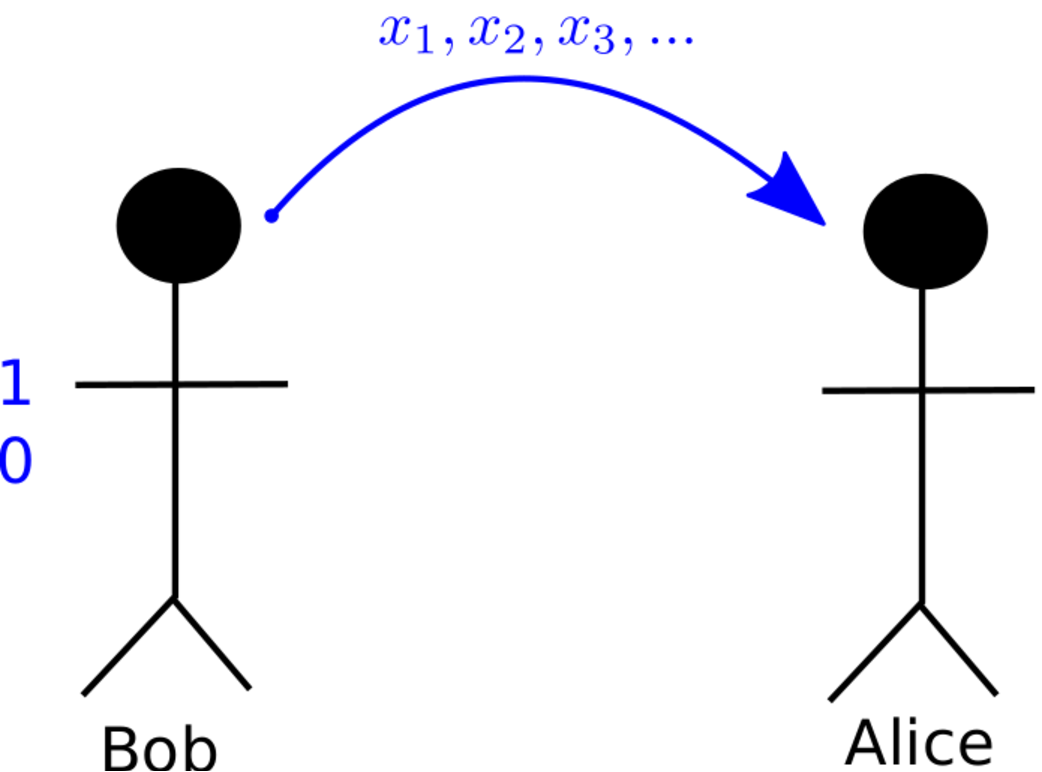
\includegraphics[height=2.5cm]{alice_and_bob_channel.pdf}
\end{figure}
\begin{block}{Shannon Entropy}
\begin{itemize}
	\item Single message replaced with message random variable $X$
	\item How informative is Bob to Alice?
	\item Expected value of Suprisal:
	{\small
	\begin{align*}
		\shannon(X) &= - \sum_{i=1}^2 P_{i} \log_2(P_{i})\\
		&= \mathbb{E}[I_2(X)]
	\end{align*}}
\end{itemize}
\end{block}
\end{frame}



\begin{frame}{Entropy}
\begin{block}{Gibbs Entropy}
\begin{figure}
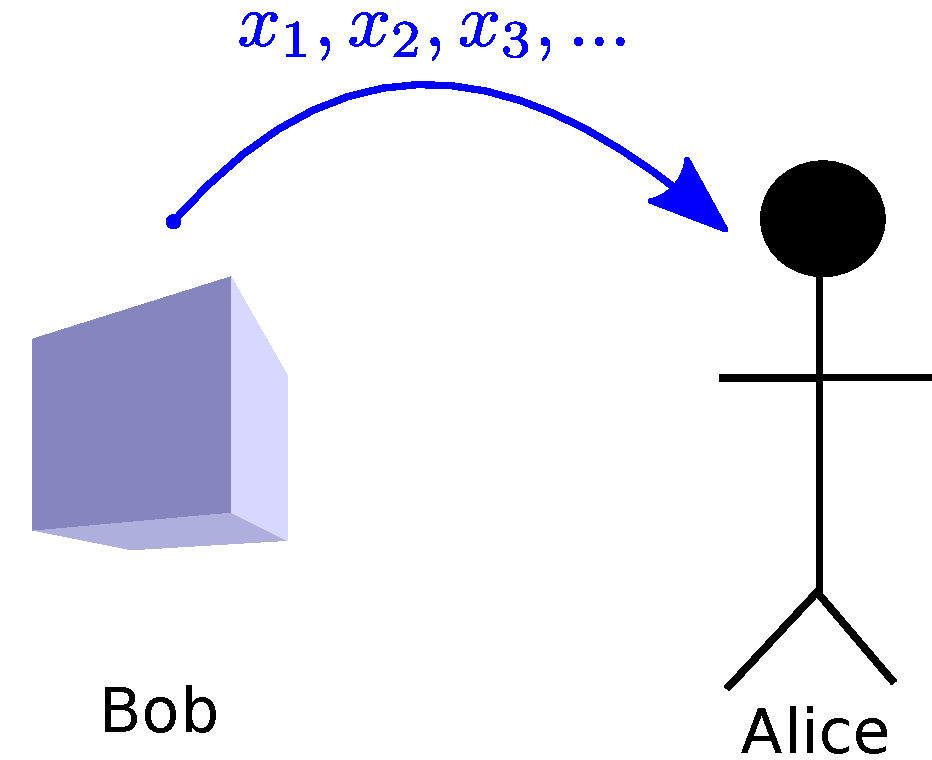
\includegraphics[height=3cm]{alice_and_bob_system.pdf}
\end{figure}
\begin{itemize}
	\item We replace the message alphabet $\Gamma$ with a finite state-space $\chi$
	\begin{align*}
		S_G &= -k \sum_{x\in\chi}P_x \ln(P_x)\\
		&= k \mathbb{E}[I_e(X)]
	\end{align*}
\end{itemize}
\end{block}
\end{frame}

\begin{frame}{Entropy}
\begin{block}{Types of Entropies Revisited}
For a system with state-space $\chi$, $x\in\chi$, and random variable $X$ with support $\chi$:
\begin{itemize}
	\item Information Content: $I_b(x) = - \log_b(P_x)$
	\item Boltzmann Entropy: $S_B = kI_e(w_0)$
	\item Shannon Entropy: $\shannon = \mathbb{E}[I_b(X)]$
	\item Gibbs Entropy: $S_B = k\mathbb{E}[I_e(X)] = k\shannon_e$ 
\end{itemize}
\end{block}
\end{frame}


\begin{frame}{Entropy}
\begin{block}{Maxwell's Demon Revisited}
\begin{itemize}
	\item Boltzmann entropy of a information-carrying bit:
	{\small
	\begin{align*}
		w_0 &= 1\\
		kI_e(1) &= -k\ln(P_1) = k\ln(2)
	\end{align*}}
	\item Boltzmann entropy of a bit overwritten with 0:
	{\small
	\begin{align*}
		w_0 &= 0\\
		kI_e(0) &= 0
	\end{align*}}
	\item Second law implies:
	{\small
	\begin{align*}
		0 &\le 0 - k\ln(2) + \Delta Q/T\\
		\implies kT\ln(2) &\le \Delta Q
	\end{align*}
	}
\end{itemize}
\end{block}
\end{frame}


















